\documentclass[11pt,a4paper]{article}
\usepackage[utf8]{inputenc}
\usepackage[spanish]{babel} 
\usepackage{fancyvrb}
\usepackage{xcolor}
\usepackage{enumitem}
\usepackage{amssymb}
\usepackage{a4wide} 
\usepackage[conEntregas]{caratula}
\usepackage{afterpage}
\usepackage{hyperref}
\usepackage{wrapfig}
\usepackage[utf8]{inputenc}
\usepackage{lmodern}
\usepackage[T1]{fontenc}
\usepackage{amsmath}
\usepackage{graphicx}
\usepackage{verbatim}
\usepackage{comment}
\usepackage{subcaption} 
\def\infinity{\rotatebox{90}{8}}
\setlength{\parindent}{12pt}
\newenvironment{metaverbatim}{\verbatim}{\endverbatim}


\begin{document}

\titulo{Trabajo Pr\'actico 2}

\fecha{\today}

\materia{Organización del Computador II}
\grupo{Grupo}

\integrante{Jim\'enez, Gabriel}{407/17}{gabrielnezzg@gmail.com}

\maketitle

\pagebreak

\section{\huge El Problema}
\noindent{\Large $\textbf{Arbitraje}$}

En el mundo de la finanzas se denomina $arbitraje$ al hecho de comprar y vender un recurso de manera simult\'anea para generar una ganancia, aprovech\'ose de los desbalances de los precios en diferentes mercados. La idea es que al ser operaciones simult\'aneas el abitrajista no corre riesgo en sus transaccciones. En genewral, los desbalances necesarios para darse una situaci\'on de arbitraje provienene de desincronizaciones de los mercados.
\\

Supongamos que hay un recurso $R$ disponible para vender y comprar en los mercados $M_{1}$ y $M_{2}$. En $M_{1}$ nos dan 36.80 pesos por vender u na unidad de $R$ u nos cuesta 37.50 pesos comprar un a unidad. En $M_{2}$ en cambio nos dan 36.90 pesos por vender una unidad  de $R$ y nos cuesta 37.65 pesos comprar una unidad. En este caso no existe oportunidad de arbitraje. No hay gorma con estos dos mercados que vendamos y compremos unidades del recurso $R$ y generemos una ganancia. Sin embargo, en un determinado momento del d\'ia sucede un evento que valoriza el recurso $R$. $M_{1}$ se entera de este suceso y actualiza sus cotizaciones. Luego de este cambio nos dan 37.67 pesos por v ender una u nidad de $R$ y nos cuesta 39.95 pesos comprar una unidad. Las noticias llegan m\'as tarde a $M_{2}$ por lo que todav\'ia no se enter\'o del suceso que valoriz\'o a $R$, por los que sus precios siguen intactos por un per\'iodo m\'as. En este caso s\'i existe oportu nidad de arbitraje.  Podemos simultaneamente comprar varias unidades del recurso $R$ en $M_{2}$ y vender varias unidades en $M_{1}$. De esta manera, por cada unidad que se compra/vende estamos obteniendo 0.02 pesos sin ning\'un tipo de riesgo.
\\

Afortunadamente, este situaci\'on, esta situaci\'on no es algo que suceda a menudo. De hecho, en el caso que suceda, muchas veces no incluye un \'unico recurso sino que involucra a varios recursos en varios mercados distintos.
\\

En este problema lo que nos gustar\'ia es si existe oportunidad de arbtiraje entre varias divisas (Pesos, D\'olares, Libras, Reales, Bitcoins, etc.). Para eso contamos con la tasa de cambio entre cada par de divisas. En caso de existir arbitraje, queremos saber qu\'e divisas son involucradas en el proceso.
\\

A continuaci\'on se expondr\'an algunos ejemplos, cada uno con su respectiva soluci\'on en caso de existir, para poder entender mejor el problema.
\\

\noindent{\large $\textbf{Ejemplo No. 1:}$} 

Para el primer ejemplo tomaremos las divisas:
\begin{itemize}
    \item[•] $d_{0}$ = D\'olares estadounidenses.
    \item[•] $d_{1}$ = Pesos argentinos.
    \item[•] $d_{2}$ = Euro.
    \item[•] $d_{3}$ = Libra esterlina.
\end{itemize}

y la "matriz de cambios" conformada por el peso de los ejes:

\[
M=
  \begin{bmatrix}
    1 & 36,64 & 0,863 & 0,760 \\
    0,027 & 1 & 0,023 & 0,020 \\
    1,159 & 42,42 & 1 & 0,88 \\
    1,315 & 48,20 & 1,136 & 1 \\
  \end{bmatrix}
\]

En la que tomaremos estos pesos como los factores multiplicativos para pasar del valor de un nodo a otro, por eso cada nodo tendr\'a distancia 1 de si mismo, entonces, si observamos el grafo asocidado a la matriz, podemos ver que este ser\'a un pseudografo dirigido completo. Ser\'a completo ya que cada divisa tendr\'a que tener un valor de cambio para otra divisa.

En resumen: $m_{i,j}$ ser\'a lo que tenga que multiplicar el valor de lo que tenga en la divisa $d_{i}$ para pasar a la divisa $d_{j}$.

El grafo asociado a nuestra matriz ser\'a:

\begin{figure}[h]
\centering 
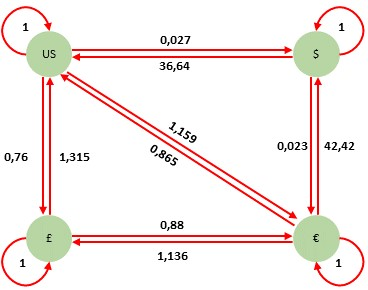
\includegraphics{Grafoejemplo2.jpg}
\end{figure}

Para que nuestro problema tenga soluci\'on debemos encontrar al menos un ciclo de divisas tales que al volver a la divisa de la que empezamos haya arbitraje.

Y, si probamos con un ciclo que empieze con  el dolar tenemos los siguientes resultados:
\begin{itemize}
    \item[•] Si el ciclo es {$d_{0}$,$d_{1}$,$d_{0}$} es decir (d  \'olares-pesos-d\'olares) tenemos que al regresar nuestra divisa valdra 1*36,64*0,027 de lo que val\'ia en un principio, es decir 0,9893 por lo tanto no se producir\'a arbitraje.
    \item[•] Si el ciclo es {$d_{0}$,$d_{2}$,$d_{0}$} es decir (d  \'olares-euros-d\'olares) tenemos que al regresar nuestra divisa valdra 1*0,863*1,159 de lo que val\'ia en un principio, es decir 1,0002: 2 diezmilesimas m\'as que antes, por lo cual aqu\'i si se producir\'a arbitraje
\end{itemize}

Como pude encontrar al menos un ciclo de divisas que me generara arbritraje, mi soluci\'on ser\'a: $d_{0}$,$d_{2}$,$d_{0}$.
\\

\noindent{\large $\textbf{Ejemplo No. 2:}$}

Para el segundo ejemplo se considerar\'a un caso en particular: cuando las divisas tienen el mismo valor de cambio entre todas. Es decir, al pasar de una moneda a otra esta sigue valiendo lo mismo. La matriz correspondiente al caso actual con 3 divisas ser\'a

\[
M=
  \begin{bmatrix}
    1 & 1 & 1 \\
    1 & 1 & 1 \\
    1 & 1 & 1 \\
  \end{bmatrix}
\]

y su pseudografo asociado
\begin{figure}[h]
    \centering
    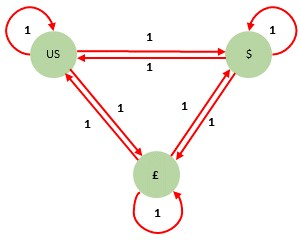
\includegraphics{Grafoejemplo1.jpg}
\end{figure}


En este caso se puede observar que ning\'un ciclo de divisas podr\'a generar alg\'un tipo de ganancia, ya que al pasar por cualquier divisa y volver a la divisa inicial esta conservar\'a su valor original, de manera que no habr\'a ganancia, pero tampoco p\'erdida. Por lo tanto podremos concluir que  no existir\'a oportunidad de arbitraje.
\\

\noindent{\large $\textbf{Ejemplo No. 3:}$}

Como \'ultimo ejemplo tendremos en cuenta el grafo en el cual $\forall$ divisa $d_{i}$ con 0 $\leq i \leq$ 3 exista un ciclo de divisas que empieza y termina en $d_{i}$ tal que haya posibilidad de arbitraje. Es decir, si tenemos la matriz
\[
M=
  \begin{bmatrix}
    1 & 1.41 & 3.14 & 1.6180 \\
    1.01 & 1 & 2,02 & 3,03 \\
    4 & 4 & 1 & 4 \\
    1.03 & 1.06 & 1.09 & 1 \\
  \end{bmatrix}
\]


Y como podemos notar seg\'un lo mencionado previamente, habr\'a  soluci\'on posible al problema y ser\'a m\'as de una. Es decir, tomando los valores de cambio, cualquier ciclo de la forma C = \{$d_{i}, d_{j},....,d_{i} \}$ cumplir\'a que genere arbitraje ya que todas las divisas ya sea para la ida o para la vuelta tienen una ganancia al realizar cualquier cambio debido a que todas las aristas que unen divisas son mayores a 1. Y como el problema se trata de responder si existe posibilidad y devolver alguno de estos ciclos, podremos devolver cualquiera de ellos y esa ser\'a la soluci\'on.
\pagebreak
\section{\huge Algoritmos y soluciones}

En la presente secci\'on se explicar\'a la idea detr\'as de cada algoritmo, como la justificaci\'on de la complejidad de cada uno. Se usar\'a pseudoc\'odigo para explicar los mismos.


Para la resoluci\'on de nuestro problema utilizaremos las siguientes definiciones:
\\

{\large $\textbf{Definicion:}$} el $\textbf{camino m\'inimo}$ entre dos vértices (o nodos) es aquel camino tal que la suma de los pesos de las aristas que lo constituyen es mínima respecto de otros caminos.
\\

{\large $\textbf{Definicion:}$} el $\textbf{Circuito M\'inimo Multiplicativo }$ de un nodo v ser\'a aquel que cumpla lo siguiente:

Si de avanzar por el camino que inicia en v, multiplicando por los factores multiplicativos(pesos de las aristas), al finalizar , se consiguiera volver a v con un valor menor al inicial, este se considerara un $\textbf{Camino M\'inimo Multiplicativo }$


Entonces, en nuestro problema, diremos que habr\'a soluci\'on si al aplicar nuestros algoritmos, al regresar por alg\'un circuito, el resultado del circuito m\'inimo de un nodo a s\'i mismo es mayor que 1.

Para la resoluci\'on del problema consideraremos dos opciones/variantes, las cuales utilizaran cada una la idea de un algoritmo de camino m\'inimo conocido.

\subsection{Primer Aproximaci\'on (Bellman-Ford)}
\subsubsection{El Algoritmo}

Para la presente aproximaci\'on del problema se tendr\'a en cuenta el algoritmo de Bellman-Ford con algunas modificaciones a fin de ser \'util con el problema de arbitraje.

    Normalmente este algoritmo se usa para calcular los caminos m\'inimos de un nodo en espec\'ifico hacia todos los nodos en un grafo. En nuestro caso, no queremos calcular eso sino alg\'un $\textbf{Camino M\'inimo Multiplicativo}$ que haya en el grafo. Por lo tanto se usar\'an las herramientas de detecci\'on presentes en el algoritmo original y la idea general del mismo para poder devolver el ciclo de divisas que genera el arbitraje. Es decir, como este algoritmo calcula el camino m\'inimo, si cambiaramos las sumas por multiplicaciones podr\'iamos calcular el camino m\'inimo multiplicativo. Y en este caso, lo que haremos es cambiar el menor por un mayor y lo que obtendremos por el algoritmo ser\'a un camino multiplicativo que "maximice".

Para facilitar la comprensi\'on del mismo se introducir\'a el pseudo-c\'odigo del algoritmo que resuelve una parte intermedia del problema.
\begin{Verbatim}[commandchars=\\\{\}]
BellmanFordArbitraje(M, s)
    n = rows(M)
    distancias(n, -INFINITO)
    padre(n, -1)
    ciclo = vacio()
    distancias[s] = 1
    cambio = true
    finished = false
    
    for(int k = 1; k < n+1 && cambio && !finished; k++)
        cambio = false
        for(int i = 0; i < n && !finished; i++)
            for(int j = 0;j < n && !finished; j++)
                \textcolor{red}{if distancias[i] * M[i][j] > distancias[j]:}
                    cambio = true
                    distancias[j] = distancias[i] * M[i][j]
                    padre[j] = i
                    if distancias[s] > 1: finished = true
                
            
    if (!cambio || distancias[s] <= 1)
        return ciclo

    comienzoCiclo =  s;
    current = comienzoCiclo
    agrego current a ciclo
    mientras current != comienzoCiclo
        agrego current a ciclo
        current = padre[current]
    agrego current a ciclo
    return ciclo
\end{Verbatim} 

Para explicar el funcionamiento de este algoritmo se tendr\'a en cuenta la utilidad de las siguientes variables:
\begin{itemize}
    \item[•] distancias: en la posicion s se guardar\'a la distancia del nodo s a s\'i mismo por alg\'un camino/ciclo.
    \item[•] padre: se utilizar\'a para reconstruir el ciclo que involucre a s en caso de exitir uno.
    \item[•] tanto cambio como finished ser\'an flags que servir\'an para terminar antes con el triple ciclo.
    \item[•] ciclo: ser\'a el ciclo que genere el arbitraje empezando desde la divisa s.
\end{itemize}
Con todo lo anteriormente dicho, podemos empezar a explicar el funcionamiento del algoritmo:

Si observamos el triple ciclo for, podemos ver que este se parece un poco al del algoritmo de Bellman-Ford sobre Matrices de Adyacencia, con las siguientes diferencias:

-En la versi\'on original el for m\'as interno de todos solo itera sobre los vecinos de i, pero en particular, como todas las divisas se pueden intercambiar entre si, el grafo ser\'a completo y los vecinos de i ser\'an todos los nodos.

-Al igual que en Bellman-Ford usaremos la idea de relajar ejes y reemplazar valores en caso de encontrar un camino mejor utilizando el nodo i como intermediario, la diferencia en este caso ser\'a que la distancia de un nodo a s\'i mismo tambien podr\'a mejorar, y esto ser\'a lo que ocurra en caso de existir posibilidad de arbitraje: Se encontr\'o un camino (en este caso ciclo) que al pasar por cierta/s divisa/s genere un valor mayor al que se encontraba originalmente. Es decir, de relajar ejes tambi\'en podr\'a resultar que la distancia de un nodo a si mismo mejore, cosa que no ocurre en el algoritmo original para caminos m\'inimos, (salvo que hayan ciclos negativos) y con mejor en este caso nos referimos a que aumente. Dicho esto podemos observar que el ciclo de divisas (empezando y terminando en s) que genere arbitraje ser\'a identificado en el triple ciclo de nuestra funci\'on intermedia mediante el mecanismo de padres. Una vez terminada la "identificaci\'on" ya sea por que hizo todas las iteraciones o por el valor de alguna flag, se proceder\'a a armar dicho ciclo.


Como se mencion\'o antes, padre servir\'a para reconstruir el ciclo que genere arbitraje luego de ejecutar este triple ciclo. Notar que los flags mencionados previamente cumplir\'an con las siguientes funciones espec\'ificas:
\begin{itemize}
    \item[•] cambio ser\'a el encargado de verificar que el vector de distancias cambie por cada iteracion en k, de  no ocurrir esto el ciclo terminar\'a. Esto nos garantizar\'a que nuestra implementaci\'on sea la optimizada, en la cual no se realizar\'an iteraciones de m\'as. Si bien esto no altera la complejidad te\'orica, ayudar\'a en cuanto a la complejidad pr\'actica.
    \item[•] finished al igual que cambio ayudar\'a a reducir la cantidad de iteraciones en caso de ocurrir lo siguiente: si la distancia del nodo s a si mismo es mayor a 1. ¿Y por qu\'e esto sirve? Simple, esto lo que nos quiere decir es que el algoritmo encontr\'o alg\'un ciclo que empieza y termina en s por lo tanto no es necesario seguir buscando otro ciclo. Al igual que antes, esto no ayuda en cuanto a complejidad te\'orica pero si en cuanto a pr\'actica.
\end{itemize}


Por lo tanto podemos decir que el algoritmo servir\'a para calcular el problema de arbitraje si la divisa pasada por par\'ametro forma parte de un ciclo que aumente el valor al volver, el cual ser\'a el resultado. Es decir, si quisi\'eramos resolver el problema sin importar desde cu\'al nodo se comienza el ciclo deber\'iamos repetir la idea para todos los nodos, lo cual ser\'a realizado por la funci\'on ArbitrajeBF:

\begin{Verbatim}[commandchars=\\\{\}]
problemaArbitrajeBF(M)
    ciclo = vacio()
    n = M.rows()
    for int i = 0; i < n; ++i 
        ciclo = bellmanFordArbitraje(M, i)
        \textcolor{red}{Si ciclo no es vacio, salgo del for.}
            
    return ciclo
\end{Verbatim}

Notar tambi\'en que nuestro algoritmo devuelve el primer ciclo que encuentre, en caso de haber uno, empezando desde el nodo 0, lo cual puede verse en nuestro pseudo-c\'odigo en color rojo.

Como efectivamente realizamos esto para cada nodo (divisa) del grafo, y fue probado que resuelve el problema en particular para un nodo, podremos decir que nuestro algoritmo final resuelve el problema de \textbf{manera exacta} para cualquier divisa del grafo.

\subsubsection{An\'alisis de Complejidad}
Para nuestro an\'alisis de complejidad podremos reutilizar complejidades te\'oricas de los algoritmos subyacentes de camino m\'inimo que usamos para resolver los problemas. En particular, podemos ver que nuestro triple ciclo del algoritmo BellmanFordArbitraje tendr\'a complejidad $\mathcal{O}$($n^{3}$) como el del algoritmo original sobre matrices de adyacencias y que lo dem\'as (asignaciones, rearmar el ciclo) tendr\'a a lo sumo complejidad $\mathcal{O}$(n) por lo tanto podemos decir que:
\begin{center}
Complejidad Te\'orica de BellmanFordArbitraje: $\mathcal{O}$($n^{3}$)
\end{center}

Y como realizamos esto una vez por cada nodo en problemaArbitrajeBF, y siendo nuestro peor caso el de que el ciclo no exista o este exista pero est\'e en el nodo n-1, podemos concluir que la complejidad te\'orica de nuestra primer aproximaci\'on al problema ser\'a:
\begin{center}
T(n) = $\mathcal{O}$($n^{3}$)*n = $\mathcal{O}$($n^{4}$)
\end{center}

\subsection{Segunda Aproximaci\'on (Floyd-Warshall)}
\subsubsection{El Algoritmo}
La idea inicial es, igual que en el de Bellman Ford, intentar modificar el algoritmo de Floyd para que "en vez de sumar, multiplique".\\
El algoritmo de Floyd se basa en el concepto de que "si el camino más corto de A a B pasa por C, entonces la distancia de A a B es la distancia de A a C más la distancia de C a B".\\
Nosotros ahora queremos encontrar el CMM (Camino Mínimo Multiplicativo) por lo tanto queremos demostrar que "si el CMM de A a B pasa por C, entonces la DMM de A a B es la DMM de A a C multiplicada por la DMM de C a B".\\
Donde DMM = Distancia Mínima Multiplicativa que es la mínima distancia de multiplicando el peso de las aristas del CMM.\\
Supongamos que el CMM(A,B) pasa por C.\\
Tenemos el CMM(A,C) con $X$ aristas que llamaremos $H_i$ con $0 \leq i < X$.\\
Tenemos el CMM(C,B) con $Y$ aristas que llamaremos $Q_i$ con $0 \leq i < Y$. \\
Tenemos el CMM(A,B) con $Z$ aristas que llamaremos $P_i$ con $0 \leq i < Z$. \\
DMM(A,C) = $\prod\nolimits H_i$\\
DMM(C,B) = $\prod\nolimits Q_i$\\
DMM(A,B) = $\prod\nolimits P_i$\\
Queremos probar que DMM(A,B) = DMM(A,C) * DMM(C,B).\\
Esto es equivalente a $\prod\nolimits P_i$ = $\prod\nolimits H_i * \prod\nolimits Q_i$\\
También es equivalente a $\prod\nolimits P_i$ = $\prod\nolimits (H \cup Q)_i$\\
Por lo tanto queremos probar que $P = H \cup Q$\\
Suponemos que esto es falso y nos quedan 3 casos:\\
1) $P \subseteq H$ \& $P \nsubseteq Q$\\
2) $P \nsubseteq H$ \& $P \subseteq Q$\\
3) $P \nsubseteq H$ \& $P \nsubseteq Q$\\
Caso 1:\\
Si esto es verdad entonces tomamos en el tramo C-B del CMM(A,B) y va a contener una distancia $d$.\\
Si $d \leq DMM(C,B)$ es absurdo por definicion de DMM!\\
Si $d > DMM(C,B)$ entonces se puede reemplazar el tramo C-B del CMM(A,B) por CMM(C,B) y obtendríamos una longitud menor del circuito, lo que probaría, pero esto es absurdo porque este ya era el CMM por lo tanto tenía distancia mínima.\\
Caso 2:\\
Es análogo al Caso 1.\\
Caso 3:\\
Es como el caso 1 y 2 juntos.\\
\\
Por lo que queda demostrado por absurdo que $P = H \cup Q$.\\
Por lo tanto la idea del algoritmo de Floyd puede utilizarse para resolver el problema del CMM.\\
También vamos a cambiar la comparación para guardarnos los máximos en vez de los mínimos así podemos obtener facilmente el resultado del ejercicio ya que el objetivo es buscar un ciclo positivo.\\
Sería exactamente lo mismo si invertimos la matriz y ejecutamos el clásico algoritmo de mínimos. Pero esto nos ayuda a evitar errores de precisión al invertir la matriz.\\ 
\\
Ahora vamos a generar un pseudocódigo para analizar los cambios que tendrían que hacerse:

\begin{Verbatim}[commandchars=\\\{\}]
FloydWarshallModificado(M)
    padres = inicializar_padres()
    
    Poner diagonal de M en 1
    
    for k = 0; k < n; k++ 
        for i = 0; i < n; i++
            for j = 0; j < n; j++
                dt = distancias[i][k] * distancias[k][j]
                if distancias[i][j] < dt
                    distancias[i][j] = dt
                    padres[i][j] = padres[k][j]
                endif
            endfor
        endfor
    endfor
    
    Recorremos la diagonal para ver si alguno quedo mayor que uno:
        Reconstruimos el ciclo a partir de ese con la matriz de padres
        Si lo logramos: ganamos! encontramos un ciclo positivo.
        
    Invertimos el ciclo (porque lo reconstruimos al reves)
\end{Verbatim}

Así es la primera idea de como sería el algoritmo. Es un típico algoritmo de Floyd-Warshall, recorre todos los nodos y para cada uno, se fija para todas las distancias si alguna se puede mejorar haciendo pasar al camino por ese nodo. La única diferencia es que ahora estamos usando multiplicación en vez de suma para poder encontrar las DMM y cambiamos la comparacion para que ahora guarde los mayores asi encontramos el ciclo positivo.\\
Luego de correr Floyd-Warshall obtenemos la matriz de distancias y la matriz de padres, pero... y el problema?...\\
Para recordar: Tenemos que obtener el ciclo.\\
Por lo tanto tenemos que recorrer la matriz de distancias y fijarnos si es que algún elemento de la diagonal dio mayor que 1.\\
Nosotros empezamos con todos 1s en la diagonal, esto quiere decir que si alguno terminó mayor eso significa que hay un ciclo que lo hizo "mejorar" de su valor original para ir a sí mísmo.\\
Si encontramos uno de estos podemos recorrer la matriz de padres comenzando en ese nodo y hacia atras para encontrar todo el ciclo.\\
Puede suceder que cuando estás recorriendo hacia atras la matriz de padres, te encuentres con otro ciclo antes de volver al nodo inicial del ciclo que estás buscando, tomamos la decision de que si esto sucede vamos a tirar a la basura el ciclo que encontramos hasta ahora y seguir recorriendo nodos de la diagonal hasta encontrar el nodo inicial del ciclo más chico y así devolver ese.\\
Finalmente damos vuelta el ciclo obtenido ya que lo reconstruimos de atrás para adelante y lo devolvemos ya que es el resultado del ejercicio.\\
\\

\subsubsection{An\'alisis de Complejidad}
Al igual que en Bellman-Ford, podremos reutilizar la complejidad te\'orica del algoritmo subyacente, el cual es sabido es $\mathcal{O}$($n^{3}$), y diremos que esta ser\'a la complejidad final ya que despu\'es del triple ciclo no hay nada que tenga mayor complejidad. Es decir:

Complejidad del triple ciclo = $\mathcal{O}$($n^{3}$).

Complejidad de llenar la matriz distancias y rearmar el ciclo en caso de existir uno = $\mathcal{O}$($n^{2}$).

Por lo tanto podemos concluir:

Complejidad Total del algoritmo = $\mathcal{O}$($n^{3}$).

\pagebreak
\section{Experimentaci\'on, An\'alisis y Conclusiones}
\subsection{Experimento de Complejidad}
Para este experimento se comparar\'an los tiempos de ejecuci\'on de cada algoritmo con su complejidad te\'orica en el peor caso.

A continuaci\'on se detallar\'a el peor caso de cada uno de los algoritmos:
Para nuestra primera aproximaci\'on (Bellman-Ford) diremos que el peor caso ser\'a aquel en el cual el ciclo que genere arbitraje sea el que involucre al \'ultimo nodo pero no a los primeros n-2 nodos. Es decir, que el ciclo de divisas sea $d_{n}-d_{n-1}-d_{n}$. Esto se deber\'a a que nuestro algoritmo hace una b\'usqueda secuencial para ver si la divisa i forma parte de un ciclo, con i = $0....n-1$.
Y en particular para nuestra segunda aproximaci\'on, diremos que su peor caso = mejor caso = caso promedio por lo tanto probaremos varios casos para ver que cumpla con la complejidad propuesta.

En particular consideraremos las siguientes instancias en base a las cuales se realizar\'a la experimentaci\'on:
Todos unos: en esta instancia todos los valores de la "matriz de cambios"  ser\'an 1, es decir: $d_{i,j}$ = 1 $\forall$ i,j. Por lo tanto $no$ habr\'a oportunidad de arbitraje.
Ciclo Cn: para esta instancia tendremos en cuenta el ciclo que contenga las n divisas como lo indica el nombre.
Ciclo $d_{n}-d_{n-1}-d_{n}$: como se mencion\'o antes, esta ser\'a el peor caso de nuestro primer algoritmo.

Notar que para toda la experimentaci\'on de complejidad se tomar\'an los siguiente valores para las variables involucradas en el problema:
\begin{itemize}
    \item[•] El valor de $n$ = cantidad de nodos/divisas ser\'a creciente empezando en 3 hasta llegar a 500.
    \item[•] En los experimentos en los que se compare un algoritmo con su complejidad te\'orica se usar\'a escala logar\'itmica a fines de que las diferencias de tiempos sean m\'as apreciables.
    \item[•] El peso de las aristas que no formen parte del ciclo ser\'a demasiado chico(Ej: 0.2, 0.0).
\end{itemize}
Para la experimentaci\'on comenzaremos con el primer algoritmo: problemaArbitrajeBF por lo que querremos formular lo siguiente:

\begin{itemize}
    \item[•] \textbf{Hip\'otesis BF:} El algoritmo que resuelve el problema de arbitraje que usa la idea del algoritmo de Bellman-Ford como intermedia tendr\'a una complejidad pr\'actica a lo sumo igual que la de su complejidad te\'orica: $\mathcal{O}$($n^{4}$)
\end{itemize}
Empezaremos con la instancia Ciclo $d_{n}-d_{n-1}-d_{n}$:
\begin{figure}[h]
    \centering
    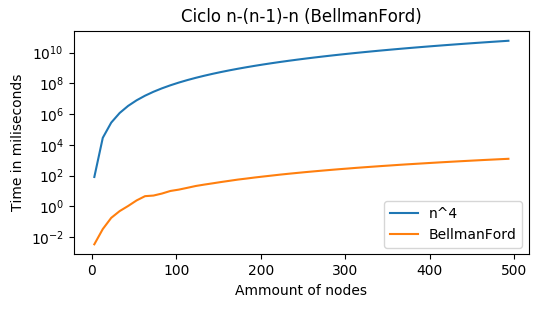
\includegraphics[height = 4.5cm,width = 9cm]{BFlog-nnl1n.png}
\end{figure}
\pagebreak

Y lo que podemos notar hasta ahora es que la cota propuesta es muy grosera. Entonces, si observamos los siguientes graficos correspondientes a la instancia Todos unos:

\begin{figure}[h]
    \caption{El primer gr\'afico (izquierda) corresponde a el tiempo de ejecuci\'on dividido por la complejidad te\'orica.}
    \caption{El segundo corresponde a las comparaciones en escala logar\'itmica.}
    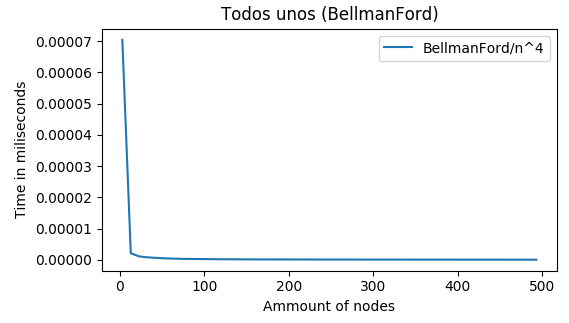
\includegraphics[height = 6cm,width = 9cm]{B-F4unos.png}
    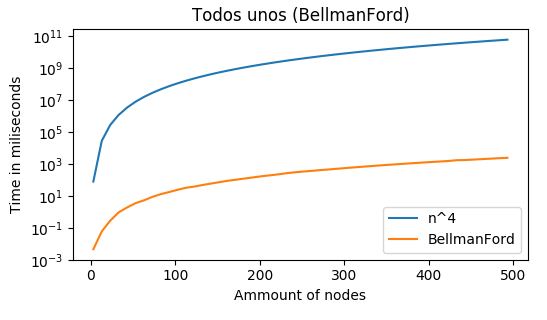
\includegraphics[height = 6cm,width = 9cm]{BFlog-unos.png}
\end{figure}

Podremos llegar a dos an\'alisis: como mencionamos antes, la cota ser\'a muy grosera y esto se puede notar en los dos gr\'aficos pero m\'as que nada en el primero, ya que de dividir nuestro tiempo de ejecuci\'on actual por la complejidad propuesta resulta una funci\'on que tiende a cero asint\'oticamente, lo cual nos indica que efectivamente $\mathcal{O}$($n^{4}$) ser\'a una cota superior.

Y lo segundo que podemos mencionar es que a diferencia de lo afirmado previamente, el caso en el que todas las divisas tienen tasa de cambio 1 entre s\'i, es peor que el caso Ciclo $d_{n}-d_{n-1}-d_{n}$.

En cuanto a lo primero, si vemos los siguientes gr\'aficos en los cuales dividimos el tiempo de ejecuci\'on del caso Todos unos por $n^{3}$ y $n^{2}$ respectivamente:

\begin{figure}[h]
    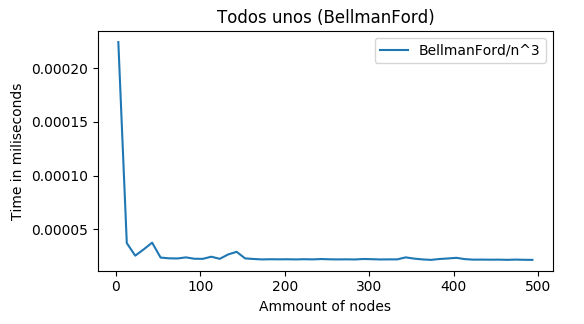
\includegraphics[height = 6cm,width = 9cm]{BF3-unos.png}
    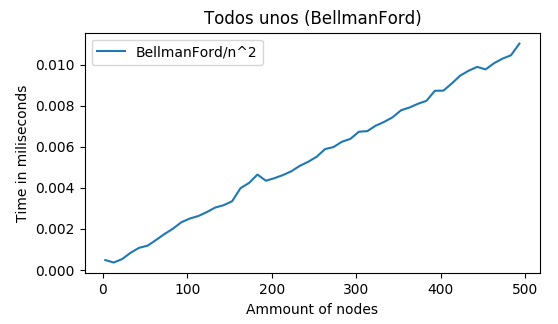
\includegraphics[height = 6cm,width = 9cm]{BF2-unos.png}
\end{figure}

Podremos ver que reci\'en cuando dividimos por $n^{2}$ tendr\'emos una funci\'on lineal que inclusive tendr\'a una pendiente muy chica lo cual confirmar\'ia que $\mathcal{O}$($n^{4}$) es una cota muy grosera pero que sigue sirviendo como cota superior.
Por lo tanto podemos concluir: nuestro algoritmo cumple que en la pr\'actica, su complejidad te\'orica es una cota superior.
\\
\begin{center}
  \rule{100mm}{0.1mm}  
\end{center}


Ahora, formularemos la hip\'otesis correspondiente a nuestra segunda aproximaci\'on:

\begin{itemize}
    \item[•] \textbf{Hip\'otesis FW:} El algoritmo que resuelve el problema de arbitraje que usa la idea del algoritmo de Floyd-Warshall como intermedia tendr\'a una complejidad pr\'actica a lo sumo igual que la de su complejidad te\'orica: $\mathcal{O}$($n^{3}$), y la complejidad pr\'actica de todos los casos (peor, mejor, promedio) ser\'a muy parecida.
\end{itemize}

Observaci\'on: Para este algoritmo usaremos todas las instancias previamente mencionadas.

Entonces, empezando con los gr\'aficos con escala logar\'itmica:


\begin{figure}[h]
    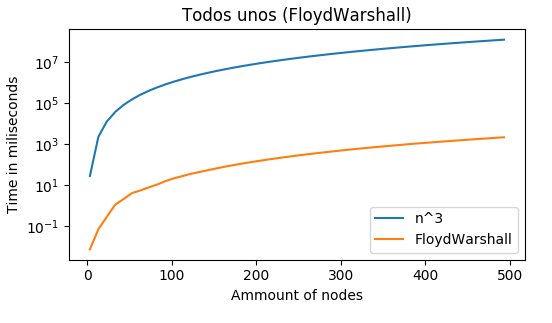
\includegraphics[width=0.55\textwidth]{FWlog-unos.png}
    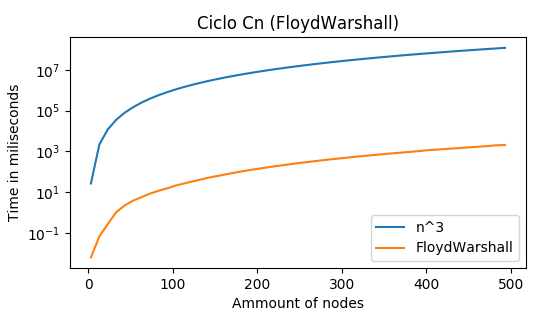
\includegraphics[width=0.55\textwidth]{FWlog-cn.png}
    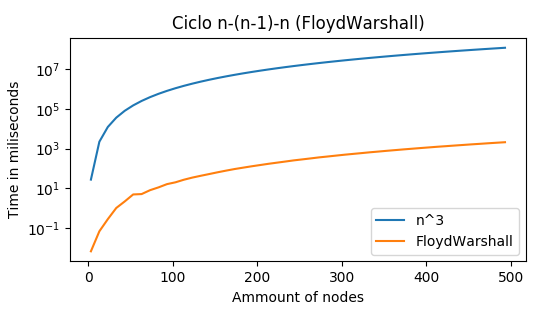
\includegraphics[width=0.55\textwidth]{FWlog-nnl1n.png}
\end{figure}

Si observamos todos estos gr\'aficos podemos observar que distintos casos de ejecuci\'on del mismo algoritmo las cuales, algunas tienen soluci\'on (Ciclo $d_{n}-d_{n-1}-d_{n}$ y Ciclo $C_{n}$) y otras no (Todos unos) tendr\'an curvas muy similares, lo cual validar\'ia la segunda parte de nuestra hip\'otesis. 

Adem\'as podemos notar que aqu\'i tambi\'en la complejidad te\'orica ser\'a una cota. Para poder ver esto mejor veremos los siguientes gr\'aficos:

 \begin{figure}[h]
     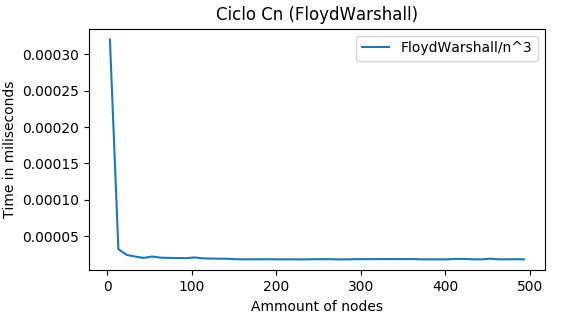
\includegraphics[height = 5cm,width = 9cm]{F-W3cn.png}
     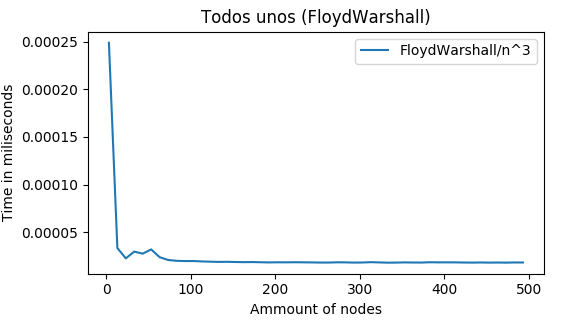
\includegraphics[height = 5cm,width = 9cm]{F-W3unos.png}
     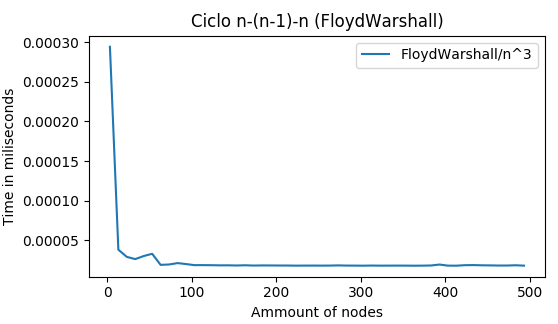
\includegraphics[height = 5cm,width = 9cm]{FW3-nnl1n.png}
 \end{figure}
 \pagebreak
 
 De lo que podremos concluir: al igual que con nuestro anterior experimento, la complejidad te\'orica ser\'a una cota superior grosera, y esto har\'a que al dividir nuestro tiempo de ejecuci\'on por la misma resulte una funci\'on que tiende a cero. Es decir, $n^{3}$ tender\'a a infinito m\'as r\'apido en tiempo de ejecuci\'on que nuestra funci\'on propuesta, lo cual nos permite asegurar que la complejidad te\'orica ser\'a una buena cota superior.

\end{document}
